\documentclass[border=10pt]{standalone}
\usepackage{pgfplots}
\pgfplotsset{compat=1.18}
\begin{document}
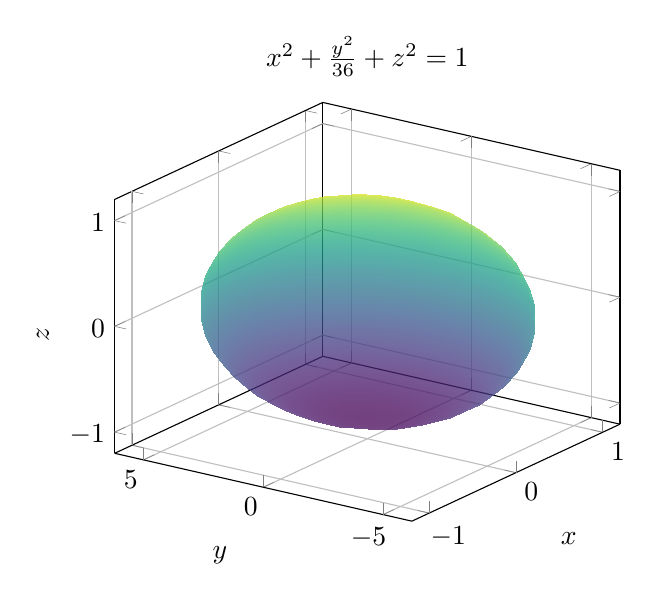
\begin{tikzpicture}
\begin{axis}[
    width=8cm,
    view={-55}{25},
    xlabel={$x$},
    ylabel={$y$},
    zlabel={$z$},
    title={$x^2+\frac{y^2}{36}+z^2=1$},
    xmin=-1.2, xmax=1.2,
    ymin=-6.2, ymax=6.2,
    zmin=-1.2, zmax=1.2,
    grid=major
]
\addplot3[
    surf,
    shader=interp,
    opacity=0.75,
    colormap/viridis,
    domain=0:360,
    y domain=0:180,
    samples=35,
    samples y=20
]
({cos(x)*sin(y)}, {6*sin(x)*sin(y)}, {cos(y)});
\end{axis}
\end{tikzpicture}
\end{document}